\documentclass[10pt]{article}
\usepackage{longtable}
\usepackage{float}
\usepackage{wrapfig}
\usepackage{rotating}
\usepackage[normalem]{ulem}
\usepackage{amsmath}
\usepackage{textcomp}
\usepackage{marvosym}
\usepackage{wasysym}
\usepackage{amssymb}
\usepackage{hyperref}
\usepackage{color,soul} % for highlighting
\usepackage{graphicx}
\graphicspath{{/Users/benjaminbass/seacloud/class/earthMaterials/picBank/}}

\usepackage{frame,color}
\usepackage{framed}
\usepackage{minibox}

% \usepackage[T1]{fontenc}
% \usepackage{tilting} %bring title up
% \setlength{\droptitle}{-10cm}

\usepackage[version=3]{mhchem}
% How to Use MChem
% \ce{SO4^2-}
% \ce{^{227}_{90}Th+}
% \ce{A\bond{-}B\bond{=}C\bond{#}D}
% \ce{CO2 + C -> 2CO}
% \ce{SO4^2- + Ba^2+ -> BaSO4 v}


\author{Benjamin Bass}
\date{15 March 2016}
\title{\vspace{-2.0cm} Beryl} %bring title up temporary Fix

\begin{document}

\maketitle

% \framebox{Use frameboxes until figure out alignmen}

\begin{center}
  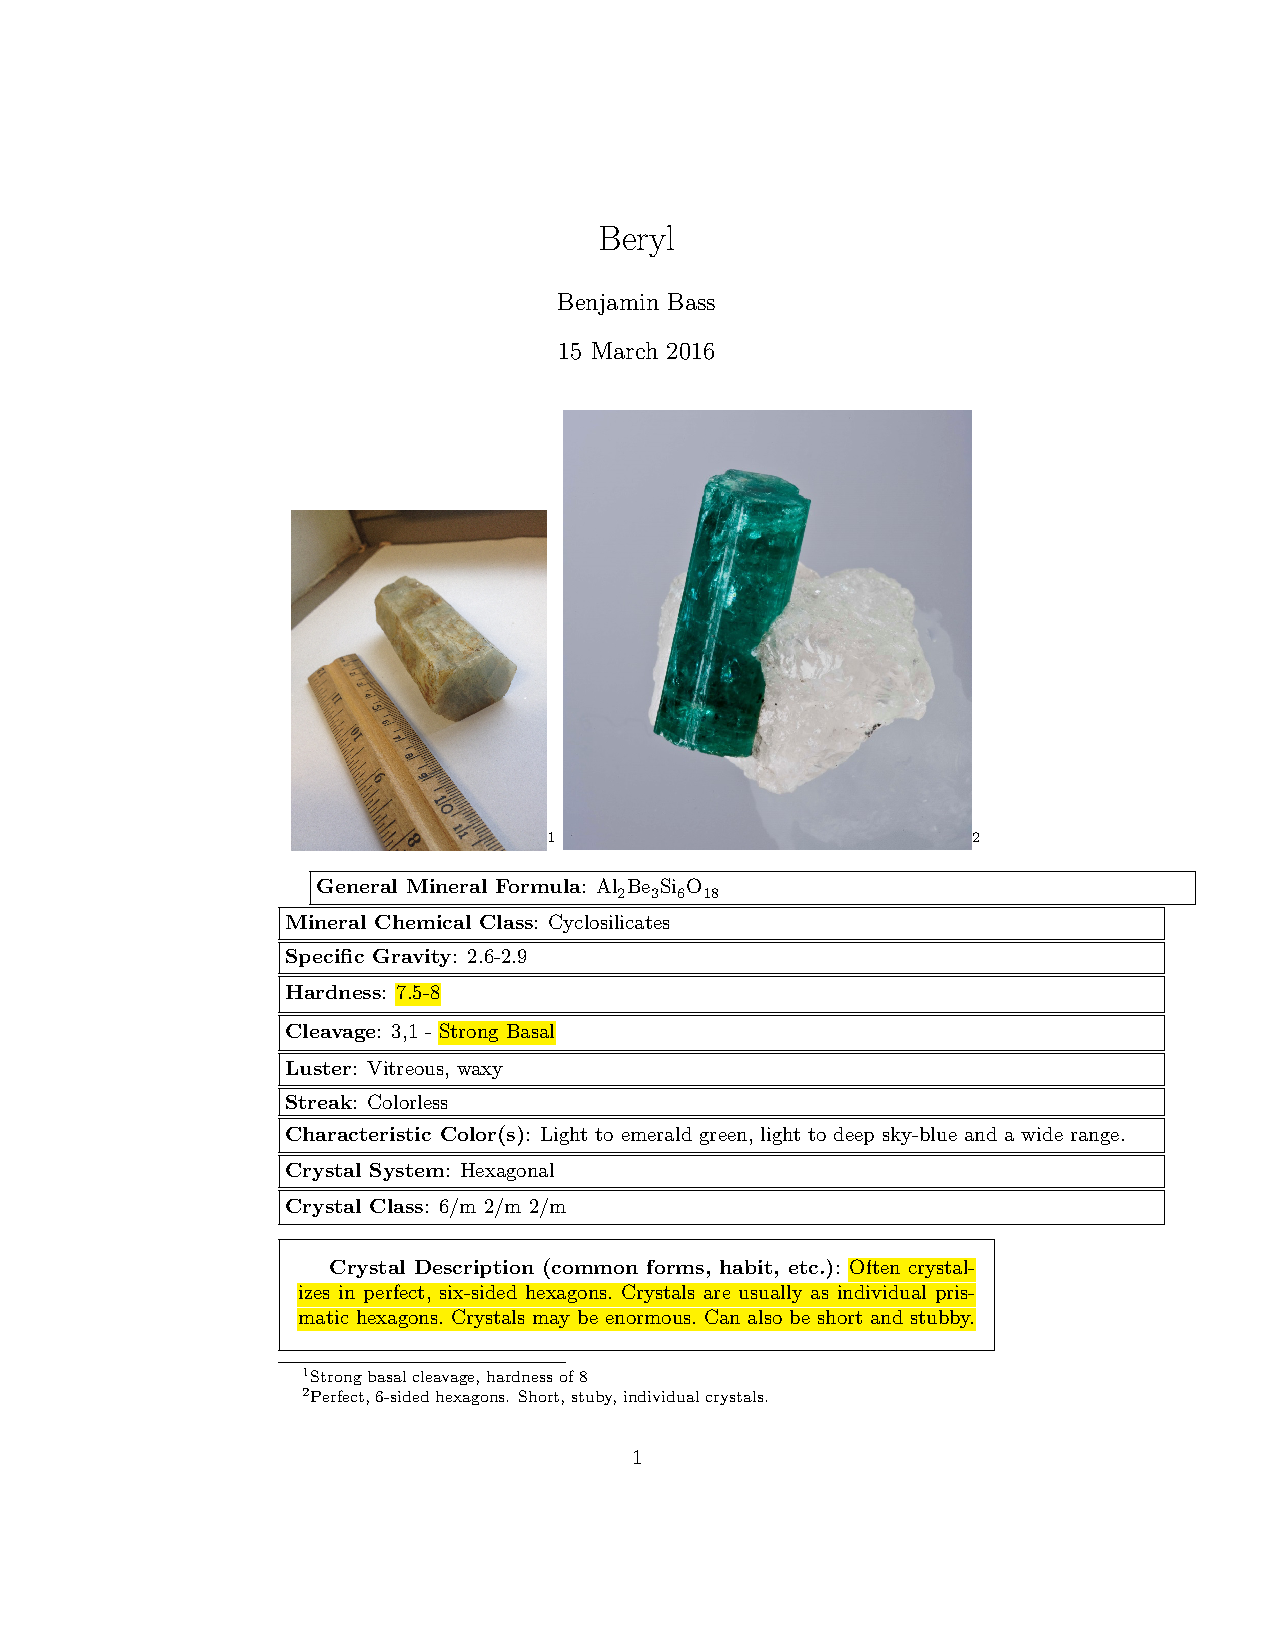
\includegraphics[scale=0.05]{beryl}\footnote{Strong basal cleavage, hardness of 8}
  \includegraphics[scale=0.75]{beryl2}\footnote{Perfect, 6-sided hexagons. Short, stuby, individual crystals.}
\end{center}



\framebox[15cm][l]{\textbf{General Mineral Formula}: \ce{Al2Be3Si6O18} }\
\framebox[15cm][l]{\textbf{Mineral Chemical Class}: Cyclosilicates }\
\framebox[15cm][l]{\textbf{Specific Gravity}: 2.6-2.9 }\
\framebox[15cm][l]{\textbf{Hardness}: \hl{7.5-8} }\
\framebox[15cm][l]{\textbf{Cleavage}: 3,1 - \hl{Strong Basal} }\
\framebox[15cm][l]{\textbf{Luster}: Vitreous, waxy }\
\framebox[15cm][l]{\textbf{Streak}: Colorless }\
\framebox[15cm][l]{\textbf{Characteristic Color(s)}: Light to emerald green, light to deep sky-blue and a wide range. }\
\framebox[15cm][l]{\textbf{Crystal System}: Hexagonal }\
\framebox[15cm][l]{\textbf{Crystal Class}: 6/m 2/m 2/m }\

\begin{framed}
  \textbf{Crystal Description (common forms, habit, etc.)}: \hl{Often crystalizes in perfect, six-sided hexagons. Crystals are usually as individual prismatic hexagons. Crystals may be enormous. Can also be short and stubby.}
\end{framed}

\begin{framed}
  \textbf{Environment (where you find the material)}: Beryl is most well-known from granite pegmatites. It can also be found in metamorphosed mica schists and in igneous rhyolite deposits.
\end{framed}

\begin{framed}
  \textbf{Common Mineral Associations (in samples, also consult text, notes}: Quartz, Muscovite, Albite, Orthoclase, Calcite, Pyrite
\end{framed}

\begin{framed}
  \textbf{Scientific Usage/Significance}: Primary source for metallic beryllium. 
\end{framed}

\begin{framed}
  \textbf{Industrial or Social Use/Significance}: Beryl with Cr is called Emerald and is a very valuable gemstone.
\end{framed}

\begin{framed}
  \textbf{Environmental Significance}: Source of Be.
\end{framed}

% Possible other Solutions
% \framebox(300,20){\minibox{\textbf{R-Sq}:For example}}

\end{document}
%%% Local Variables:
%%% mode: latex
%%% TeX-master: t
%%% End:
